\chapter{Methodology}
\label{ch:methodology}

This chapter outlines the methods used to analyze the security and potential vulnerabilities of the Anapaya version of SCION.
The general approach is presented in \cref{sec:general-approach}, followed by the concrete setup used in the assessment in \cref{sec:setup}.
\cref{sec:analysis-methods-tools} provides an in-depth look at the methods and tools used in the analysis.
Finally, \cref{sec:methodology:disclosure} describes the disclosure process with Anapaya.


\section{General Approach}
\label{sec:general-approach}
The general approach of this thesis focuses on a comprehensive analysis of the security features and potential vulnerabilities of the Anapaya version of SCION.
Given its proprietary nature, this research employs a combination of exploratory and analytical approaches.

\subsection{Exploratory Approach}
The exploratory approach is utilized in this research to address the limited public knowledge about Anapaya's version of SCION.
As this version incorporates proprietary modifications that are not fully publicly documented, an exploratory approach is essential for uncovering and understanding these new or undocumented features.
The exploratory phase involves conducting preliminary investigations to identify potential vulnerabilities, security features, and other relevant aspects of the implementation.
This includes a review of available documentation, security scans, and configuration checks to gather initial data on the system.

These early findings from exploratory efforts will guide the subsequent analytical phase of the research, providing a foundation for more in-depth analysis and testing.

\subsection{Analytical Approach}
The analytical approach is employed to systematically evaluate and interpret the security characteristics identified during the exploratory phase.
This approach is crucial for conducting a detailed analysis of the security mechanisms and potential vulnerabilities within the Anapaya SCION environment.
It involves a detailed examination of the identified security mechanisms, potential vulnerabilities, and their implications for the overall security of the SCION network.
The goal is to move beyond initial discovery to a deeper understanding and rigorous assessment of security aspects.


\section{Setup}
\label{sec:setup}
The security analysis is conducted against the SCION deployment at the CYD Campus locations.
A simplified network setup is shown in \cref{fig:network-setup}.
Each CYD Campus location forms its own AS and includes an Anapaya EDGE device.
The three ASes are connected via three different Core ASes to the SCION production network.
In each of these CYD Campus ASes, we deploy a Kali virtual machine (VM) that runs the SCION end host code, enabling interaction with the SCION network.
At ETH Zurich, SCION access extends beyond the CYD Campus, where we operate an additional Kali VM.
To assess the influences of the traditional Internet on SCION, we also have access to a non-SCION VM in the ETH Zurich network.
According to the service offer from SWITCH the traditional Internet and SCION connection in Zurich are physically separated.
At the other CYD Campus locations, no such separation information is provided.

\begin{figure}[h]
    \centering
    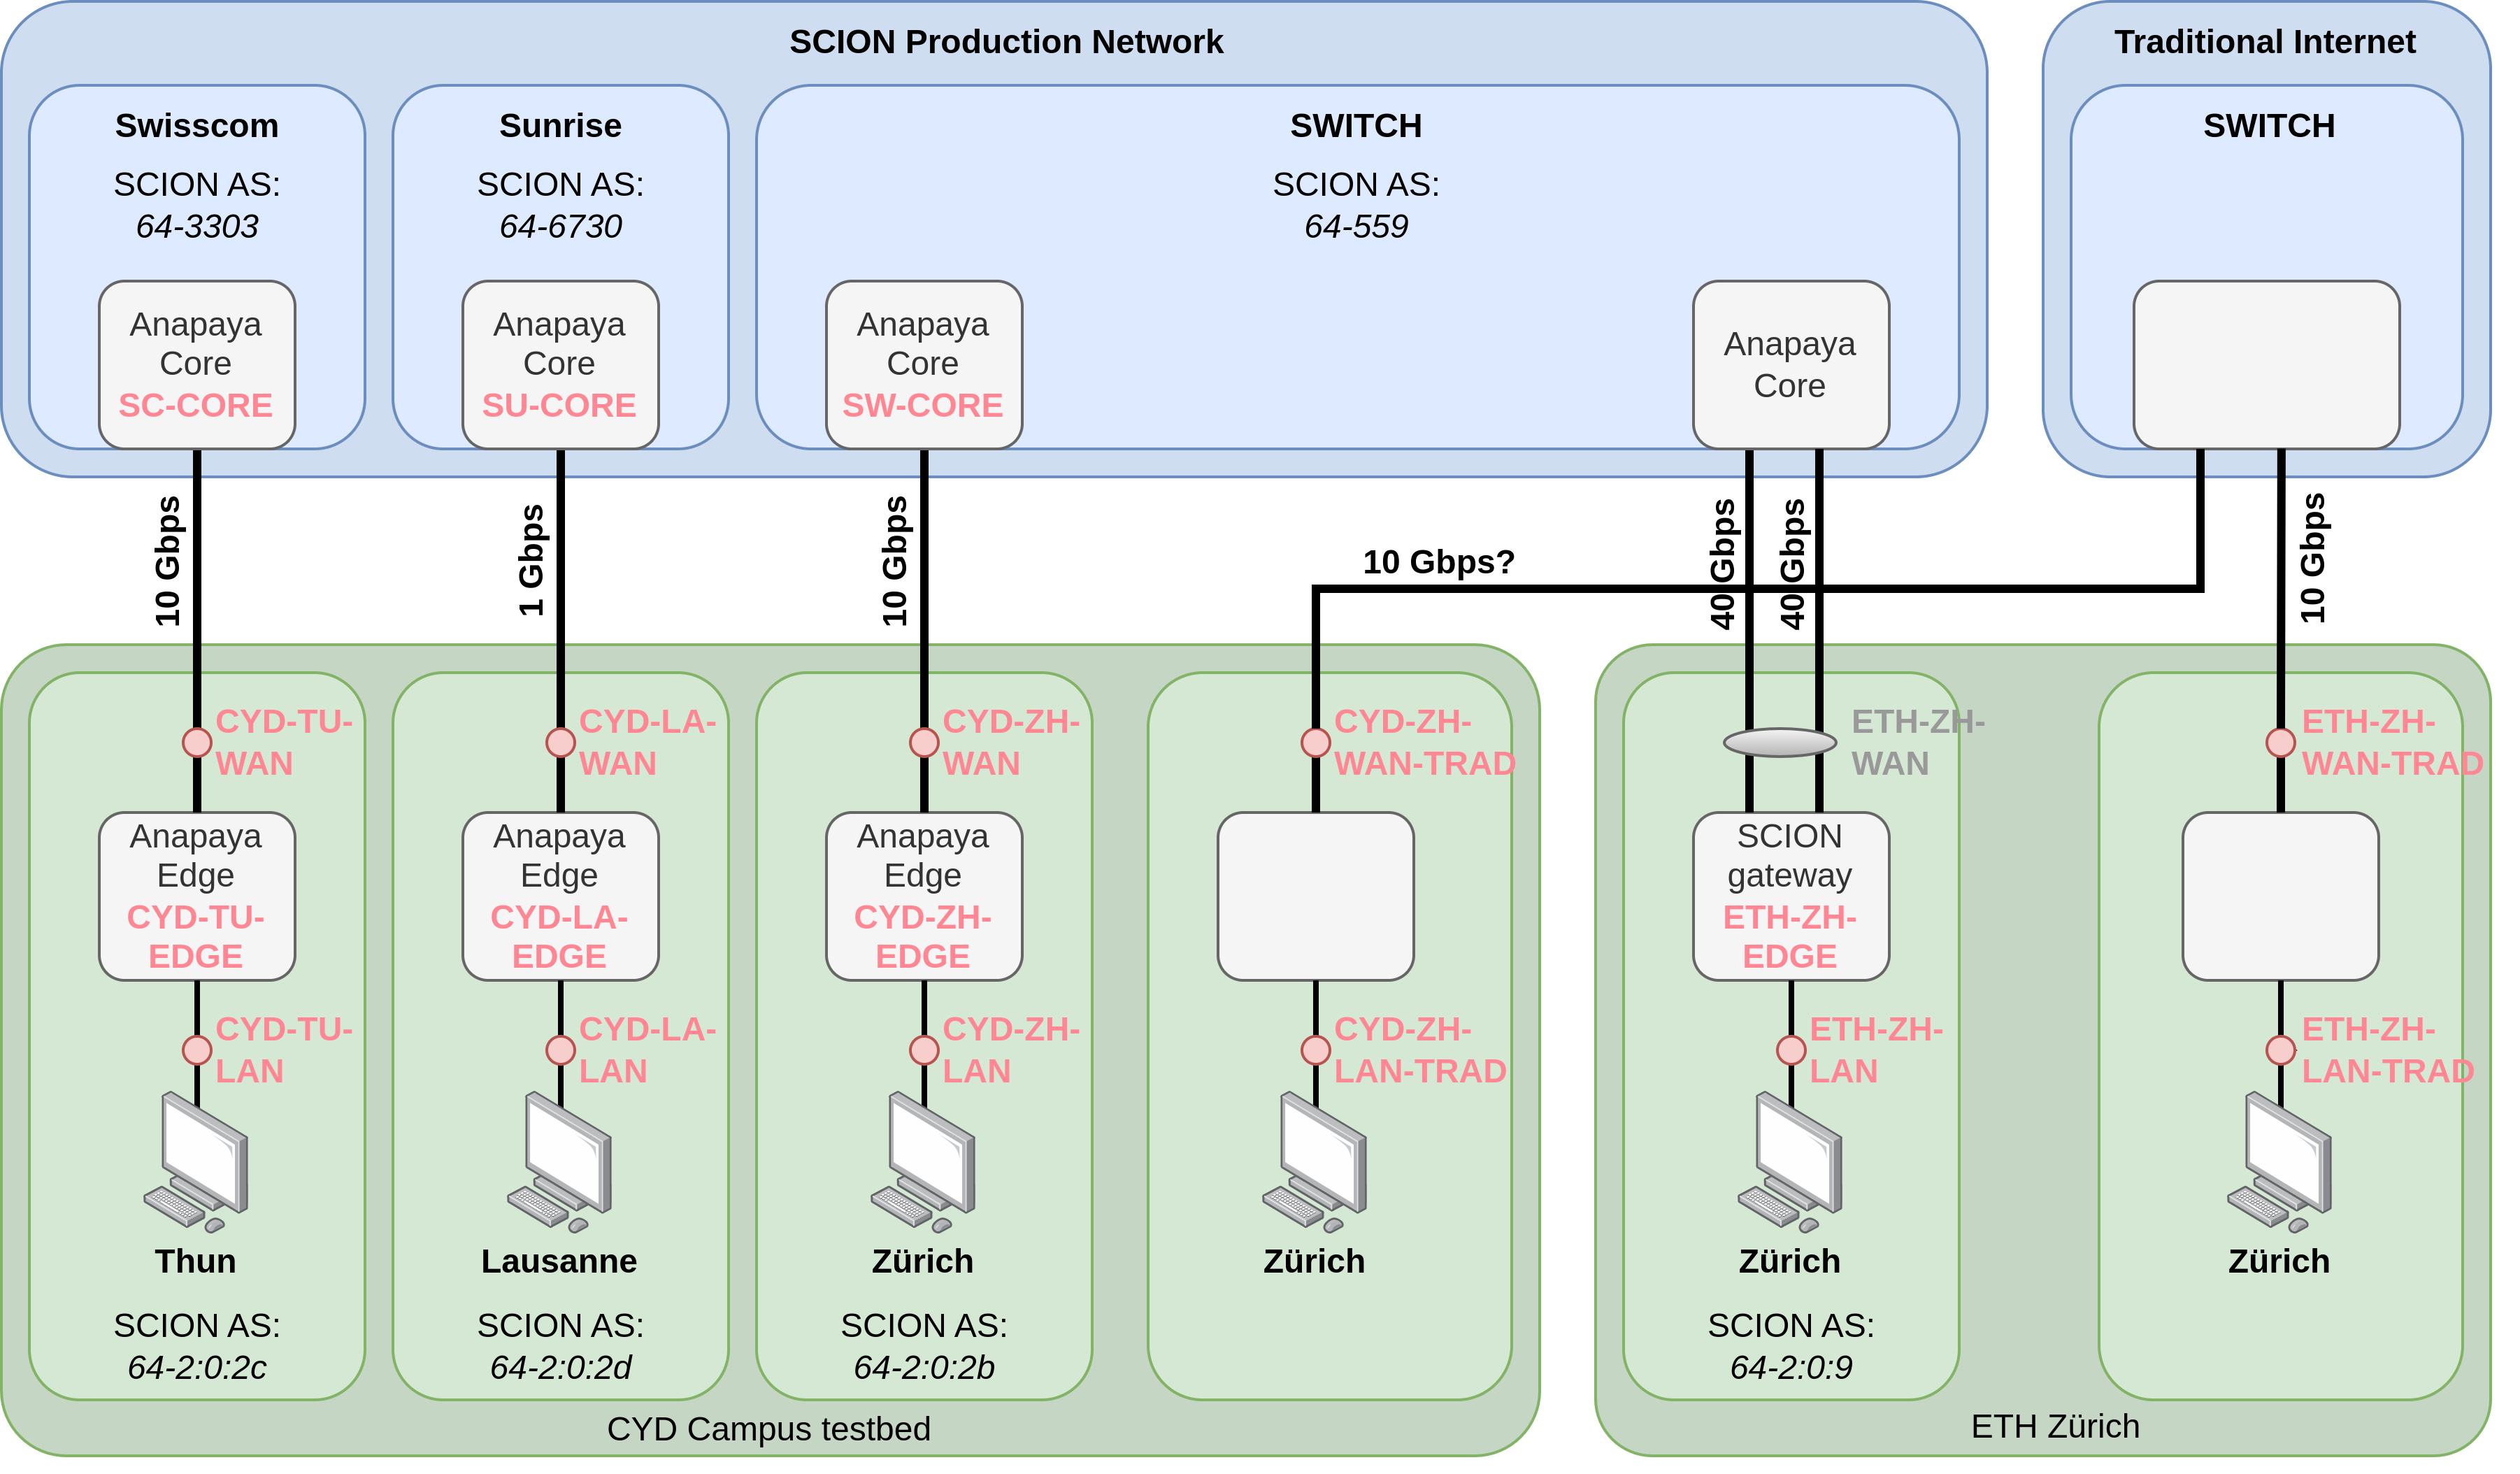
\includegraphics[width=\textwidth]{figures/scion_setup2.drawio.png}
    \caption{Network Setup during the Security Assessment}
    \label{fig:network-setup}
\end{figure}

Additionally, apart from these operational devices, CYD Campus acquired another Anapaya device.
It is not part of the SCION production network and only used for offline testing purposes.

\newpage
\section{Analysis Methods and Tools}
\label{sec:analysis-methods-tools}
This section outlines the methods and tools used to conduct the security analysis of the Anapaya EDGE devices.

\subsection{Automatic Scans}
To conduct our exploratory analysis, we employ automated scanning tools to identify potential vulnerabilities and security weaknesses in the deployed Anapaya devices.
The popular tools \textbf{Nessus} and \textbf{OpenVAS} give an initial overview of the security posture of the devices by scanning for known vulnerabilities and misconfigurations.
Nessus is also being used to perform a compliance audit to check if the devices adhere to security best practices and standards, such as CIS benchmarks.
An \textbf{SSH audit} is conducted to identify potential weaknesses in the SSH configuration of the devices.
Furthermore, running software and services are analyzed using tools like \textbf{systemd-analyze} \cite{systemdAnalyze} and \textbf{Docker Trivy} \cite{trivy}.


\subsection{Manual Investigations}
Complementing the automated scans, manual investigations include reviewing the findings of the automated tools and conducting in-depth analysis of specific areas.
In addition, we review manually the software and configurations detected by the automated scans.

Apart from the device itself, everything related to the SCION protocol is manually checked.
This includes the SCION management system, and all SCION network interactions.
How we capture and analyze these interactions is described in the next section.


\subsection{Data Collection and Modification}
During the security analysis, network packets are generated, captured, analyzed, and modified.
This is done to observe and reason about network flows, for example to check if a reflection attack worked or not.
Furthermore, if our generated packets cause SCMP error messages, we can reason about the correct behavior or can also use this information to analyze and revise our generated packets.
We use \textbf{Wireshark/tshark} \cite{wireshark} for packet capture because there already exists a SCION plugin for Wireshark, which allows us to dissect SCION packets \cite{wiresharkSCION}.
To generate and modify SCION packets, the tools \textbf{scapy} \cite{scapy} with its SCION extension \cite{scapySCION} are used.
It allows to easily define correctly formatted SCION packets and modify them as needed.

\newpage

\subsection{Volumetric Data Generation}
We assess the robustness of SCION by conducting volumetric denial-of-service attacks.
The primary objective of such an attack is to saturate the target's network bandwidth, overwhelming it with a large volume of data packets.
For generating the volumetric data, we use the \textbf{TRex} traffic generator \cite{trexWebsite}, a versatile and high-performance tool capable of simulating both stateful and stateless traffic.
TRex allows customizing traffic parameters, enabling us to closely mimic real-world attack scenarios.
We configure TRex to send a continuous stream of large data packets, thereby maximizing the use of on network resources.
This approach allows us to evaluate the resilience of the SCION architecture under severe traffic conditions, offering valuable insights into its performance and robustness.

\section{Disclosure Process}
\label{sec:methodology:disclosure}

The disclosure process followed a structured and collaborative approach with Anapaya to ensure both thorough evaluation and responsible communication of findings.
Initially, we conducted independent penetration tests on the SCION infrastructure at the CYD Campus to identify potential security vulnerabilities and assess their impact.
This independent assessment aimed to provide an unbiased analysis of the system.
Following these tests, we held a discussion with Anapaya to share our preliminary findings and to obtain their insights and feedback.
Anapaya then implemented necessary software updates to address the identified weaknesses and vulnerabilities.
They were also given the opportunity to review and comment on the findings.
We incorporated their feedback into the final report, ensuring that their perspectives and any additional insights were accurately reflected.
Finally, Anapaya approved the publication of the results, allowing us to share the outcomes of the security analysis with the broader community.

